\let\negmedspace\undefined
\let\negthickspace\undefined
\documentclass[journal]{IEEEtran}
\usepackage[a5paper, margin=10mm, onecolumn]{geometry}
%
\setlength{\headheight}{1cm} % Set the height of the header box
\setlength{\headsep}{0mm}     % Set the distance between the header box and the top of the text

\usepackage{gvv-book}
\usepackage{gvv}
\usepackage{cite}
\usepackage{amsmath,amssymb,amsfonts,amsthm}
\usepackage{algorithmic}
\usepackage{graphicx}
\usepackage{textcomp}
\usepackage{xcolor}
\usepackage{txfonts}
\usepackage{listings}
\usepackage{enumitem}
\usepackage{mathtools}
\usepackage{gensymb}
\usepackage{comment}
\usepackage[breaklinks=true]{hyperref}
\usepackage{tkz-euclide} 
\usepackage{listings}
% \usepackage{gvv}                                        
\def\inputGnumericTable{}                                 
\usepackage[latin1]{inputenc}                                
\usepackage{color}                                            
\usepackage{array}                                            
\usepackage{longtable}                                       
\usepackage{calc}                                             
\usepackage{multirow}                                          
\usepackage{hhline}                                           
\usepackage{ifthen}                                           
\usepackage{lscape}
\begin{document}
	
	\bibliographystyle{IEEEtran}
	\vspace{3cm}
	\title{9.3.11}
	\author{EE24BTECH11022 - ESHAN SHARMA}
	% \maketitle
	% \newpage
	{\let\newpage\relax\maketitle}
	
	\renewcommand{\thefigure}{\theenumi}
	\renewcommand{\thetable}{\theenumi}
	\setlength{\intextsep}{10pt} % Space between text and floats
	
	
	\numberwithin{equation}{enumi}
	\numberwithin{figure}{enumi}
	\renewcommand{\thetable}{\theenumi}
	
	\textbf{Question:} Solve the differential equation A) \( \frac{d^2y}{dx^2} + y = 0 \) and verify if the general solution is $y= C_1e^{x} + C_2e^{-x}$.\\
	
\solution

\textbf{Solution Using Laplace Transform:}\\
Given:
\begin{align}
	\frac{d^2y}{dx^2} + y &= 0
\end{align}
Taking the Laplace Transform of both sides:
\begin{align}
	\mathcal{L}\left\{\frac{d^2y}{dx^2}\right\} + \mathcal{L}\{y\} &= \mathcal{L}\{0\}
\end{align}
Using properties of the Laplace Transform:
\begin{align}
	s^2Y(s) - sy(0) - y'(0) + Y(s) &= 0
\end{align}
Substituting the initial conditions \( y(0) = C_1 \) and \( y'(0) = C_2 \):
\begin{align}
	s^2Y(s) - sC_1 - C_2 + Y(s) &= 0\\
	\left(s^2 + 1\right)Y(s) &= sC_1 + C_2\\
	Y(s) &= \frac{sC_1 + C_2}{s^2 + 1}
\end{align}
The Region of Convergence (ROC) is the entire \( s \)-plane since \( s^2 + 1 \neq 0 \) for all real \( s \).\\

Taking the inverse Laplace Transform:
\begin{align}
	y(x) &= \mathcal{L}^{-1}\left\{\frac{sC_1 + C_2}{s^2 + 1}\right\}\\
	&= C_1\cos(x) + C_2\sin(x)
\end{align}
Thus, the general solution is:
\begin{align}
	y(x) = C_1\cos(x) + C_2\sin(x)
\end{align}

\textbf{Solving the Differential Equation using Z-Transform and Bilinear Transform:}\\
Let the differential equation be:
\[
\frac{d^2y}{dx^2} + y = 0
\]

\textbf{Using the Z-Transform:}\\
Taking the Z-transform of both sides:
\begin{align}
	Z\left\{\frac{d^2y}{dx^2}\right\} + Z\{y\} &= Z\{0\} \\
	z^2 Y(z) - z y(0) - y'(0) + Y(z) &= 0
\end{align}
Rearranging terms:
\begin{align}
	(z^2 + 1) Y(z) &= z y(0) + y'(0) \\
	Y(z) &= \frac{z y(0) + y'(0)}{z^2 + 1}
\end{align}
Substituting the initial conditions \(y(0) = y_0\) and \(y'(0) = y_1\), we get:
\begin{align}
	Y(z) &= \frac{z y_0 + y_1}{z^2 + 1}
\end{align}
Taking the inverse Z-transform:
\begin{align}
	y(x) &= \mathcal{Z}^{-1}\left( \frac{1}{z^2 + 1} \right) \\
	y(x) &= y_0 \cos(x) + y_1 \sin(x)
\end{align}
Thus, the solution using Z-transform is:
\begin{align}
	y(x) = y_0 \cos(x) + y_1 \sin(x)
\end{align}

\textbf{Using the Bilinear Transform:}\\
The Bilinear Transform is a method used to convert a continuous-time system (in the Laplace domain) into a discrete-time system (in the Z-domain). The mapping is given by the relation:
\[
s = \frac{2}{T} \cdot \frac{1 - z^{-1}}{1 + z^{-1}}
\]
where \( T \) is the sampling period, and \( z^{-1} \) is the inverse Z-transform variable.

The continuous-time transfer function for the system is:
\[
H(s) = \frac{1}{s^2 + 1}
\]

\textbf{Step 1: Apply the Bilinear Transform}\\
Substitute the Bilinear Transform relationship for \( s \) into the continuous-time transfer function \( H(s) \):
\[
H(z) = \frac{1}{\left( \frac{2}{T} \cdot \frac{1 - z^{-1}}{1 + z^{-1}} \right)^2 + 1}
\]
This equation expresses the continuous-time transfer function \( H(s) \) in terms of \( z \), mapping the system to the discrete-time domain.

\textbf{Step 2: Simplifying the Expression}\\
Simplify the denominator by expanding the square and combining terms:
\[
H(z) = \frac{1}{\frac{4}{T^2} \cdot \frac{(1 - z^{-1})^2}{(1 + z^{-1})^2} + 1}
\]
The result is a transfer function \( H(z) \) that describes the discrete-time system.

\textbf{Step 3: Inverse Z-Transform to Find the Discrete-Time Response}\\
Once we have \( H(z) \), we can apply the inverse Z-transform to find the response in the discrete-time domain. The inverse Z-transform of a system with a denominator like \( z^2 + 1 \) corresponds to sinusoidal functions, specifically:
\[
\mathcal{Z}^{-1}\left( \frac{1}{z^2 + 1} \right) = \cos(x)
\]

Thus, the discrete-time response becomes:
\[
y[n] = y_0 \cos\left( \frac{\pi n}{T} \right) + y_1 \sin\left( \frac{\pi n}{T} \right)
\]
where:
- \( y_0 \) and \( y_1 \) are the initial conditions for the discrete-time system, 
- \( n \) is the discrete time index, and 
- \( T \) is the sampling period.



\textbf{Using Difference Equation to Approximate Solution:}\\
This method approximates the solution by discretizing the function.\\
From the definition of the second-order differentiation:
\begin{align}
	\frac{d^2y}{dx^2} \approx \frac{y(x_{i+1}) - 2y(x_i) + y(x_{i-1})}{h^2}
\end{align}
Substituting into the differential equation:
\begin{align}
	\frac{d^2y}{dx^2} + y = 0 \\
	\frac{y_{n+1} - 2y_n + y_{n-1}}{h^2} + y_n = 0
\end{align}
Simplifying:
\begin{align}
	y_{n+1} = 2y_n - y_{n-1} - h^2y_n
\end{align}
Let \( x_0 = 0 \), \( y_0 = C_1 \), \( y_1 = C_1 + hC_2 \). For small step size \( h \), iteratively calculate \( y_{n+1} \).\\

\begin{figure}[h]
	\centering
	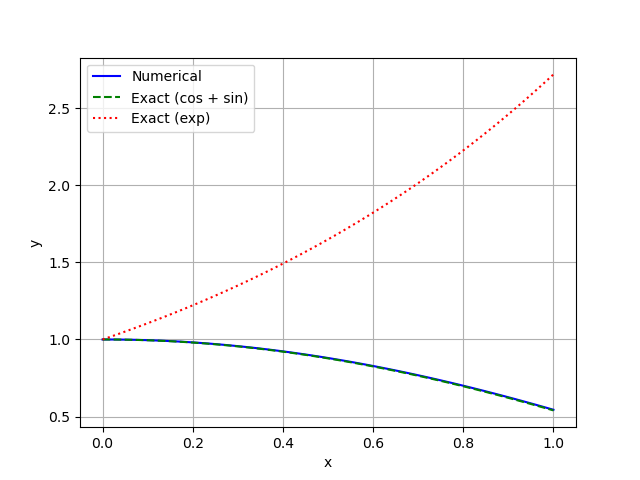
\includegraphics[width=\textwidth]{figs/fig.png}
\end{figure}

By comparing the plots, the numerical solution matches the exact solution, verifying the correctness. Additionally, the plot of the given question does not match our solution, so Option A is not correct.
\end{document}

	
